\chapter{Experiment}
\label{chapter:experiment}

After architecture of StreamBench and design of workloads are demonstrated, this chapter will draw our attention to experiments. First of all, we briefly introduce our experiment environment, its hardware configuration and software setup. Then, we present benchmark results for three stream processing systems: Storm, Flink, and Spark Streaming of three workloads discussed in~\cref{section:workloads}. As discussed in \cref{section:log_statistic}, two performance metrics that we concerned are latency and throughput. We also compare the experiment results of each workload with visualization of these two metrics. 

\section{Experiment Environment}

\label{section:cpouta}
\subsection{Hardware}

The experiment environment is a cloud service called cPouta which is the main production IaaS cloud at CSC -- a non-profit, state-owned company administered by the Ministry of Education and Culture. In cPouta,  there are several available virtual machine flavors. Each visual machine used in our experiment has 4 CPU cores, 15GB RAM, 10GB root disk and 220GB ephemeral disk. The experiment environment consists of two clusters: compute cluster and Kafka cluster. Computer cluster consists of 8 work nodes and one master nodes. Kafka cluster has 5 brokers with one zookeeper instance running on the same machine with one Kafka broker. The cPouta service is based on the hardware of the Taito cluster. Communication among nodes and to the storage is done by Infiniband FDR fabric, which provides low latency and high throughput connectivity. The detail information about hardware and inter connection could be found online~\footnote{\url{https://research.csc.fi/taito-supercluster\#1.1.2}}.

\subsection{Software}
The operator system running on experiment nodes is Ubuntu 14.04 LTS. Benchmarked stream processing systems are Spark-1.5.1, Storm-0.10.0 and Flink-0.10.1. To enable checkpoint feature of Spark, Hadoop2.6(HDFS) is installed in compute cluster. Kafka 0.8.2.1 is running as distribute message system here.

\section{WordCount}
First, we examined workload WordCount which aims to evaluate performance of stream processing systems performing basic operators. To check different aspects of stream processing systems, we performed three different versions experiments of WordCount: Offline WordCount, Online WordCount and Windowed WordCount. Offline WordCount focus on throughput and aims to find the corresponding maximum throughput of each systems. Offline means that the workload application consumes data that already exist in Kafka. On the contrary, experiments consuming continuous coming data are called Online WordCount, which measures both latency and throughput. Moreover, in~\cref{subsection:window_wordcount} we also made some modification to the original workload to evaluate pre-aggregation property of Storm. 


As mentioned in~\cref{subsection:wordcount_generator}, for this workload, we designed two data generators: uniform generator and skewed generator. In our experiments, for both generators, the number of words in each sentence satisfies normal distribution with mean as 10 and sigma equals to 1. The interval of uniform distribution in uniform generator is \texttt{[1,10000]}.  The parameters of zipf distribution in skewed generator are \texttt{size:10000} and \texttt{skew:1}.


\subsection{Offline WordCount}
\begin{figure}[t!]
  \begin{center}
  \subfigure{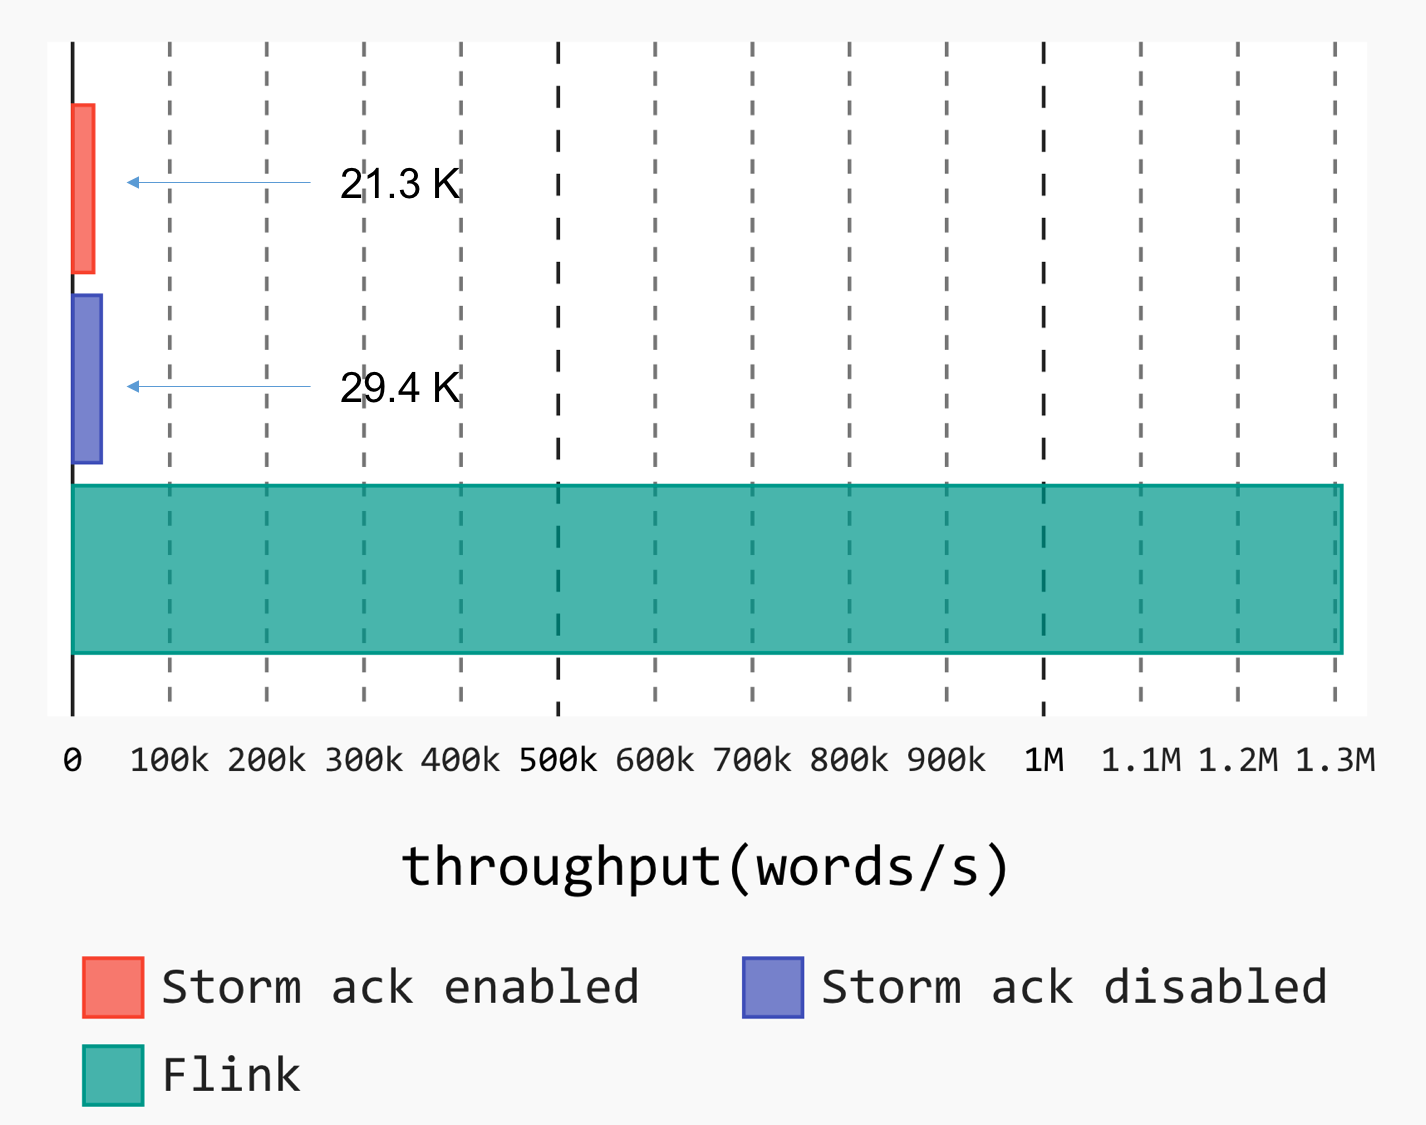
\includegraphics[scale=0.2]{images/throughput_skewed}}
  ~
  \subfigure{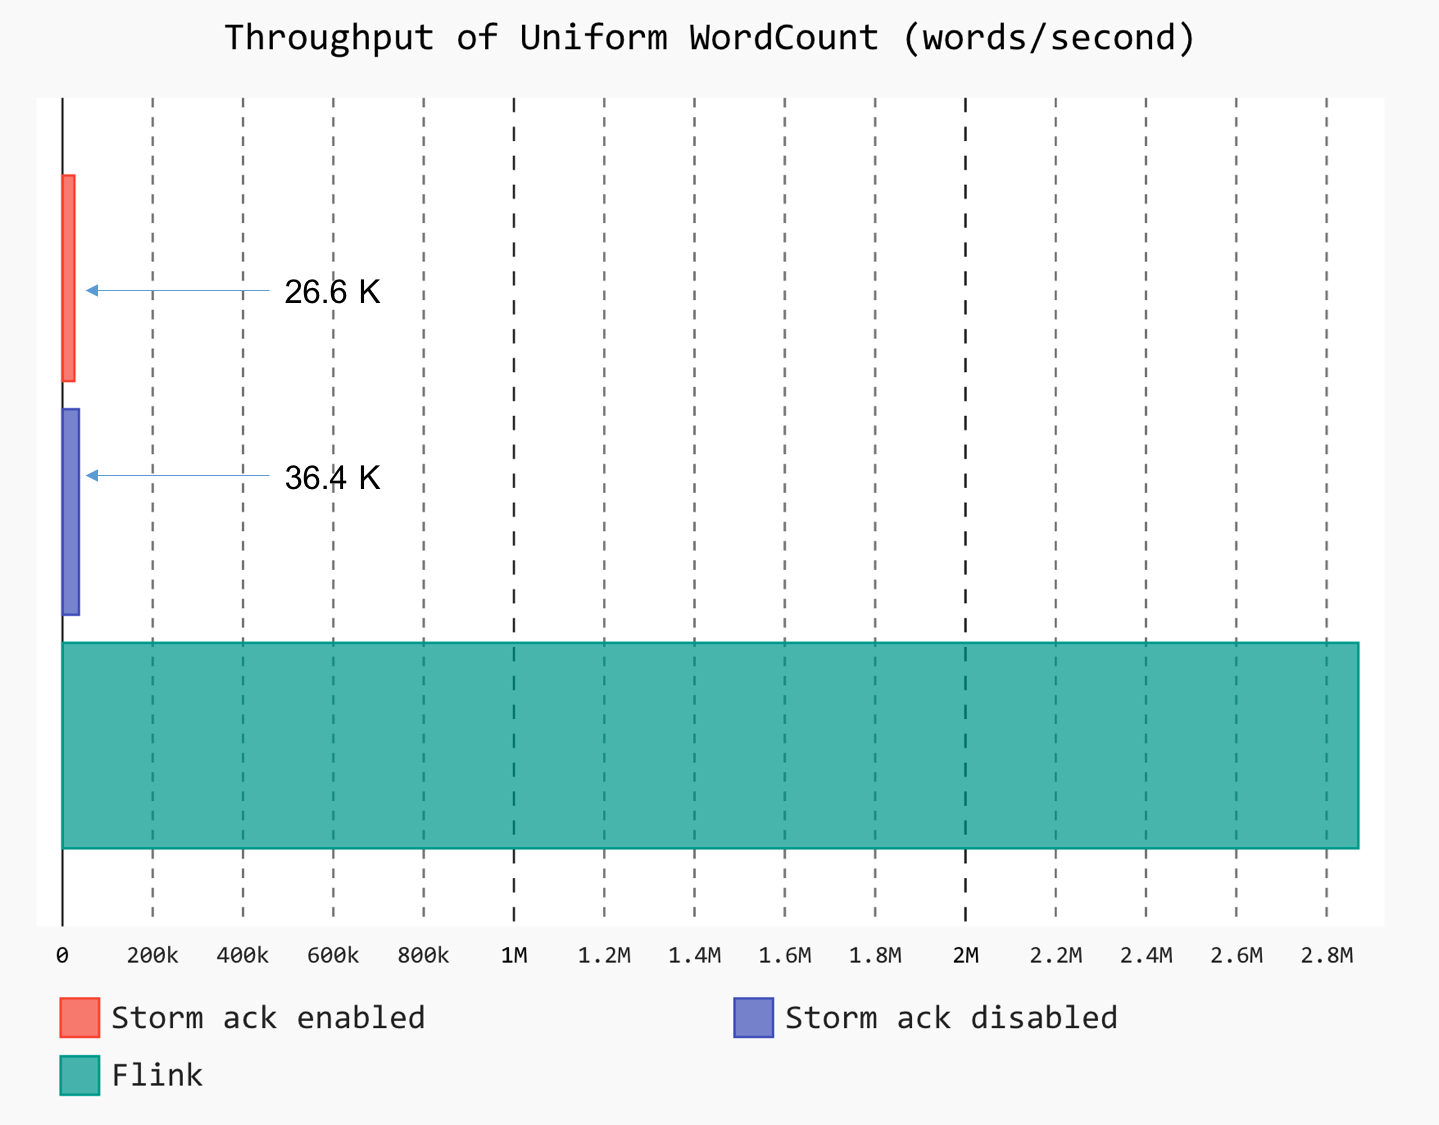
\includegraphics[scale=0.2]{images/throughput_uniform}}
   \caption{Throughput of Offline WordCount}
   \label{fig:offline_throughput}
  \end{center}
\end{figure}

Since the computing model of Spark Streaming is micro-batch processing. Existing data in Kafka would be processed as one single batch. The performance of processing one large batch with Spark Streaming is similar to Spark batch jobs. Therefore, we skipped Spark Streaming here. Figure~\ref{fig:offline_throughput} shows cluster throughput of Offline WordCount for both skewed data and uniform data. Obviously, in both experiments the throughput of Flink is much better than Storm, around 50 to 100 times larger. The skewness of experiment data has great influence of performance. The throughput of Flink cluster performing uniform data is more than two times of performing skewed data. The corresponding ratio of Storm is around 1.5. 

\begin{figure}[t!]
  \begin{center}
  \subfigure{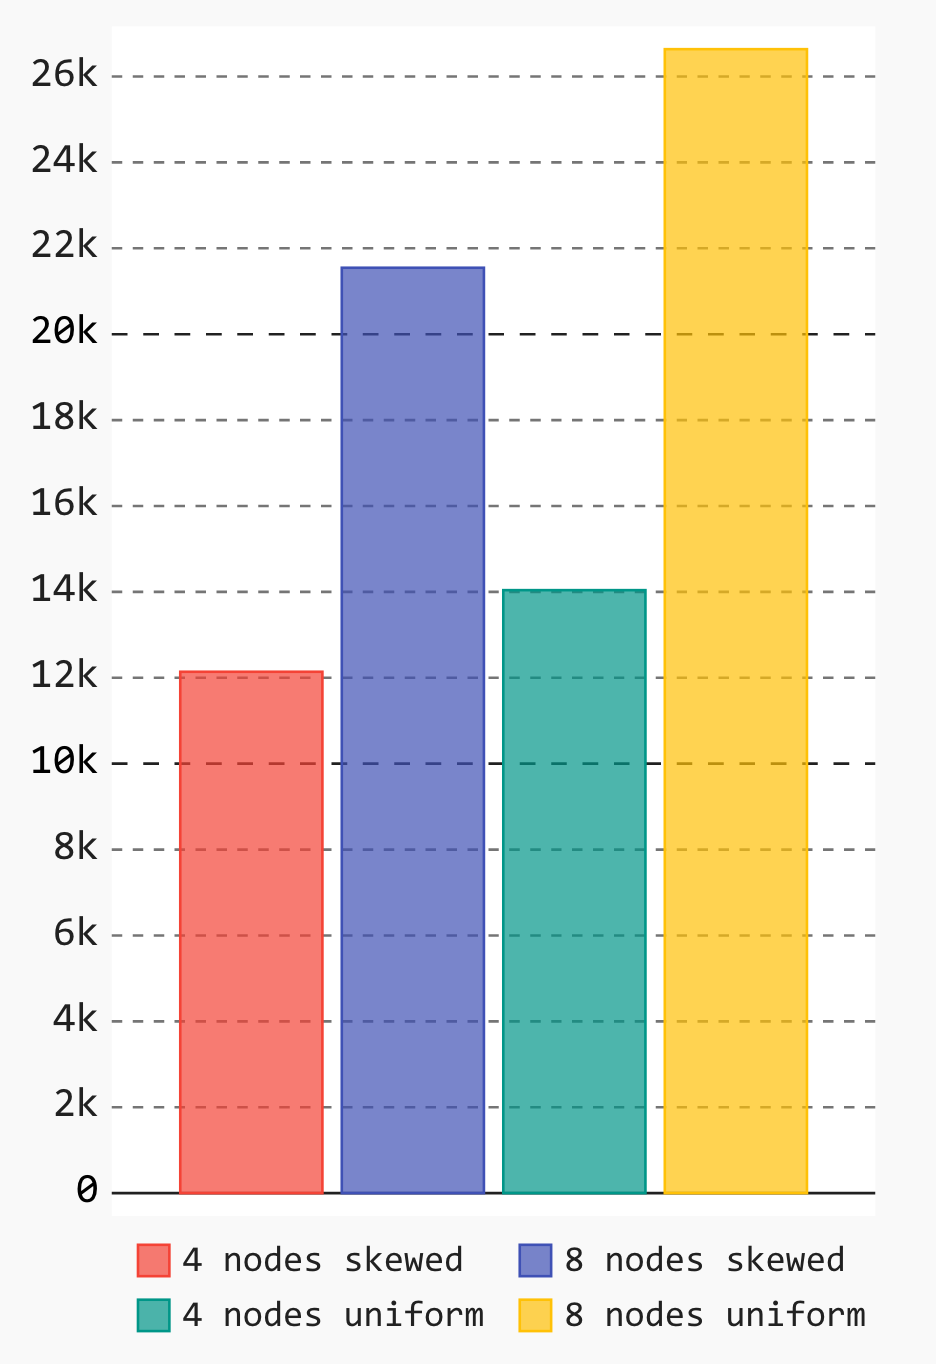
\includegraphics[scale=0.28]{images/storm_throughput_scale}}
  ~
  \subfigure{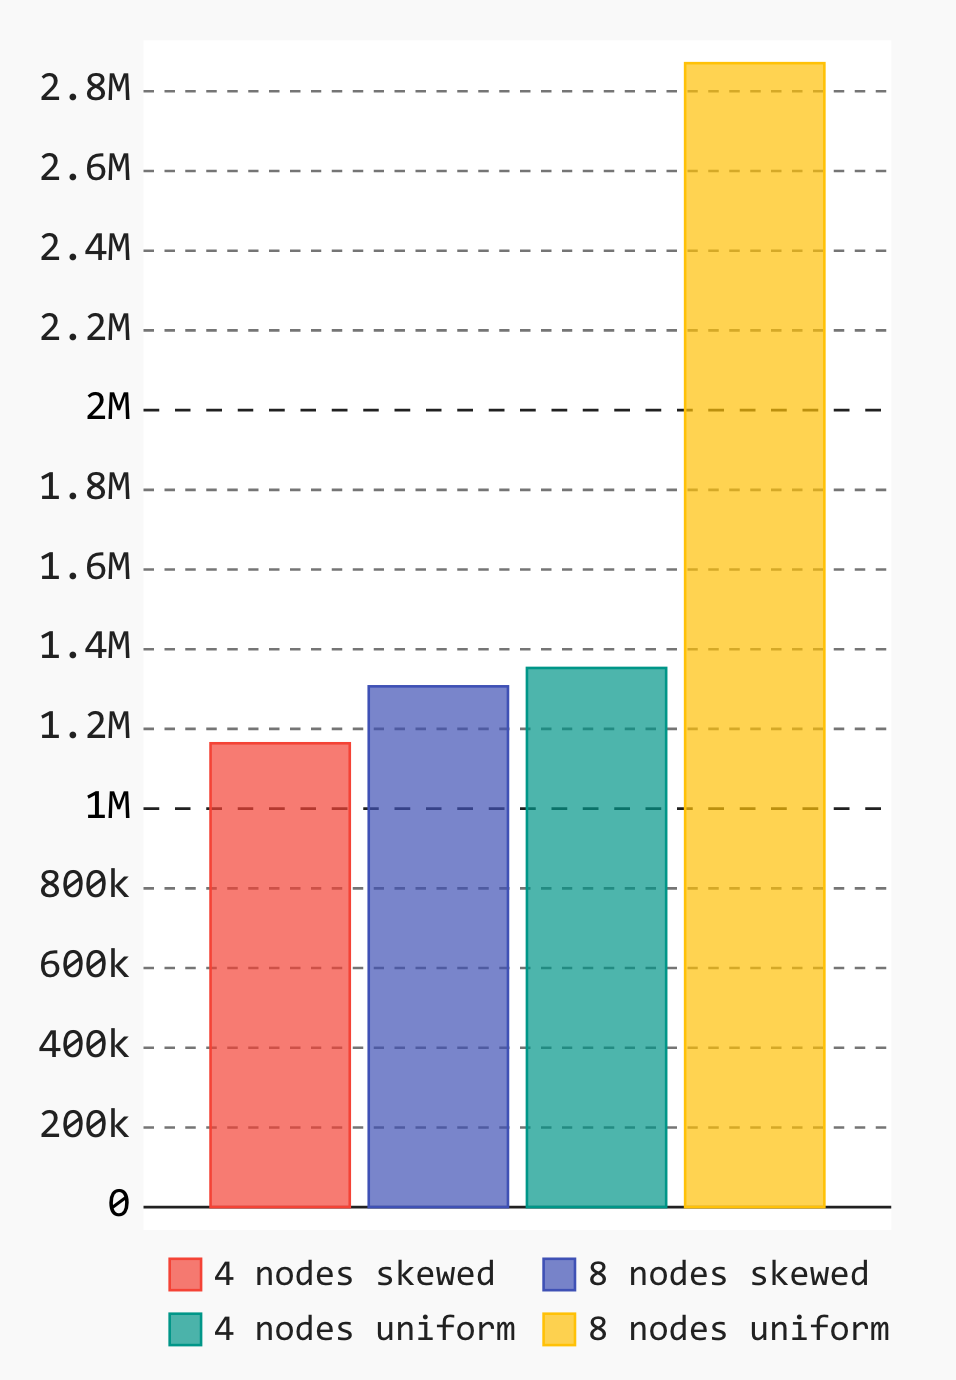
\includegraphics[scale=0.28]{images/flink_throughput_scale}}
   \caption{Throughput Scale Comparison of Offline WordCount}
   \label{fig:offline_throughput_scale}
  \end{center}
\end{figure}

The experiment results of scalability are presented as Figure~\ref{fig:offline_throughput_scale}. The throughput of 8-nodes cluster of both systems dealing with uniform data is nearly two times of that of 4-nodes cluster. That means the scalability of both system is good. While processing skewed data, increasing the number of work nodes in a Flink cluster doesn't bring significant performance increase. Storm cluster gets about 58\% throughput improvement while increasing cluster from 4 nodes to 8 nodes.

The throughput of each work node in computing cluster is displayed in Figure~\ref{fig:worknodes_throughput}. Obviously storm has lower throughput, but achieves better workload balance than Flink. The experiment results also shows that clusters with 4 compute nodes of both systems have better workload balance than clusters with 8 nodes and workloads preforming uniform data achieve better balance that corresponding workloads performing skewed data.


\begin{figure}[t!]
  \begin{center}
   \subfigure{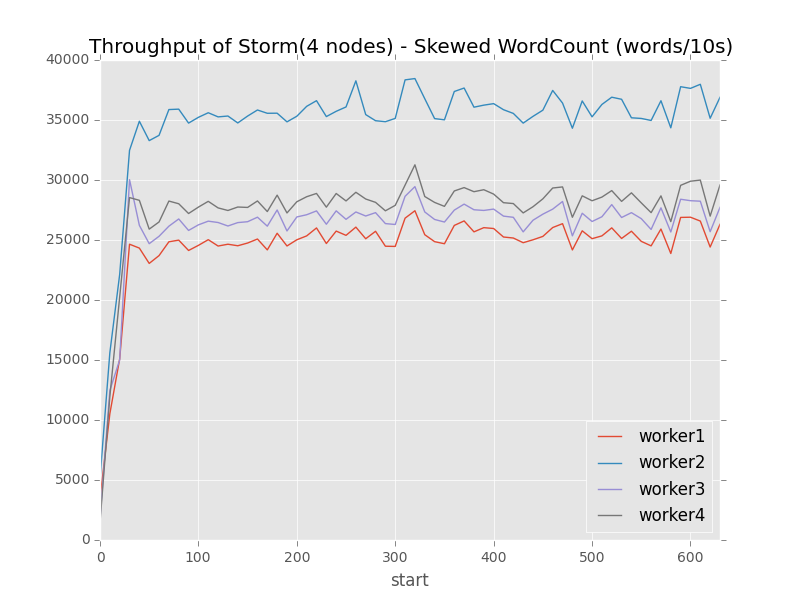
\includegraphics[scale=0.25]{images/storm4nodes_skewed_throughput}}
  ~
  \subfigure{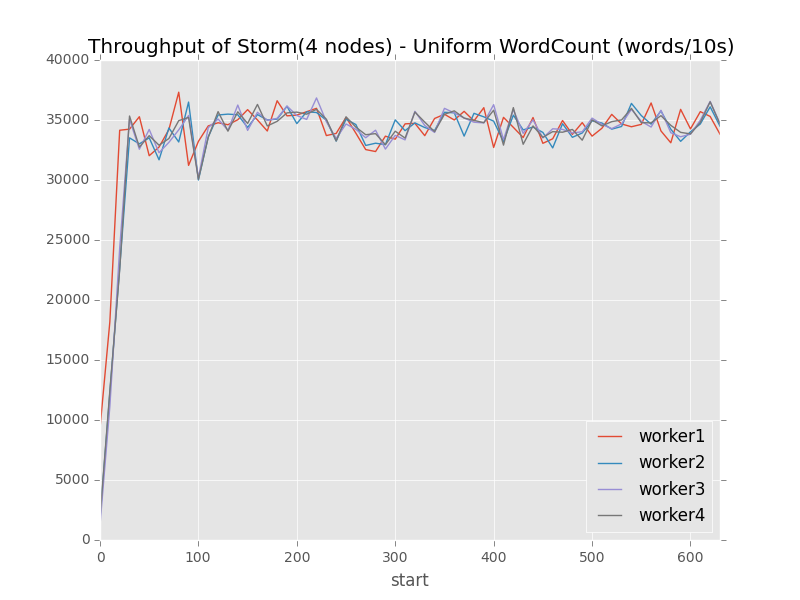
\includegraphics[scale=0.25]{images/storm4nodes_uniform_throughput}}
  ~
  \subfigure{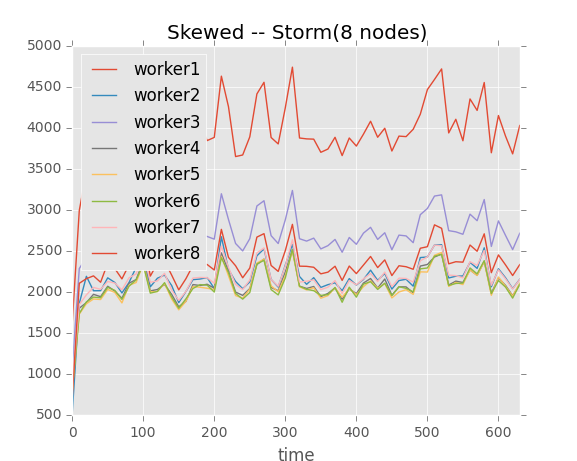
\includegraphics[scale=0.25]{images/storm_skewed_throughput2}}
  ~
  \subfigure{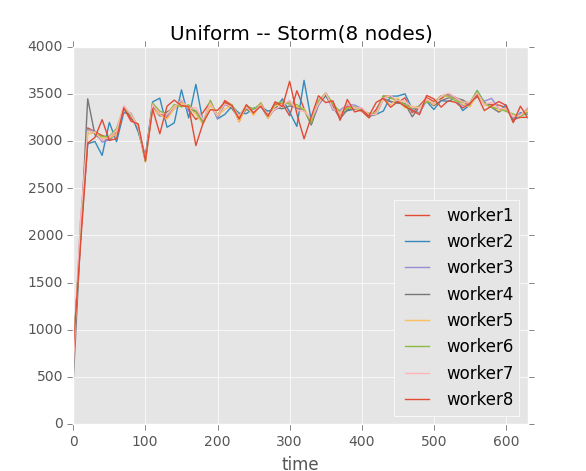
\includegraphics[scale=0.25]{images/storm_uniform_throughput2}}
  ~
    \subfigure{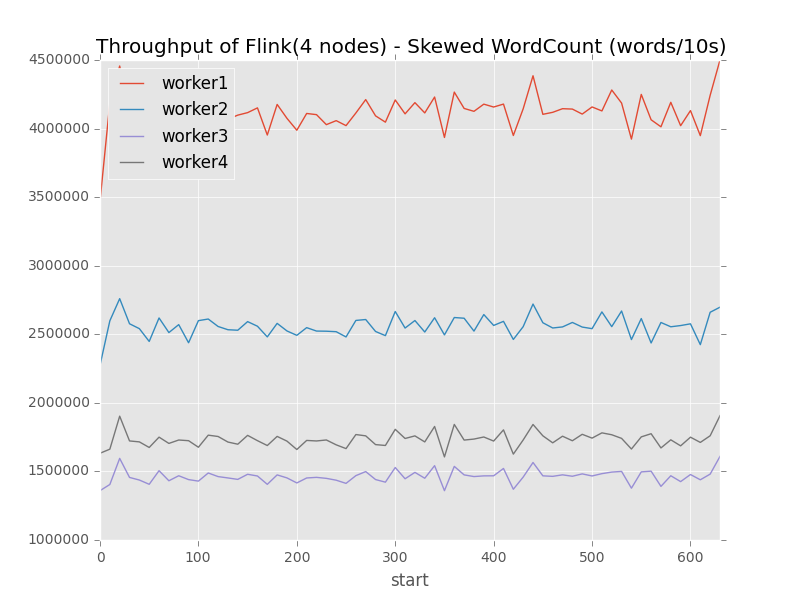
\includegraphics[scale=0.25]{images/flink4nodes_skewed_throughput}}
  ~
  \subfigure{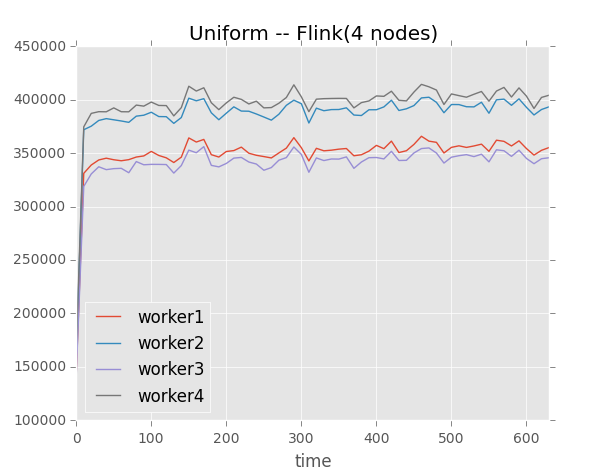
\includegraphics[scale=0.25]{images/flink4nodes_uniform_throughput}}
  ~
  \subfigure{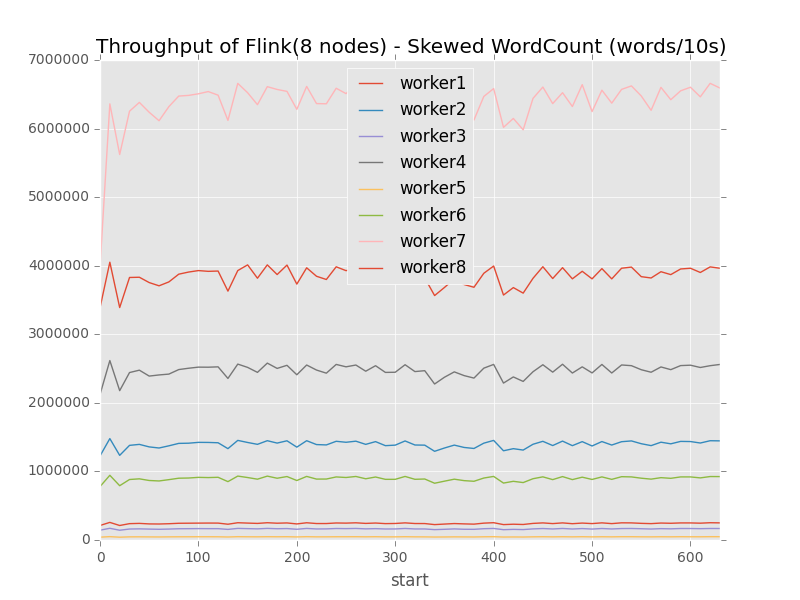
\includegraphics[scale=0.25]{images/flink_skewed_throughput}}
  ~
  \subfigure{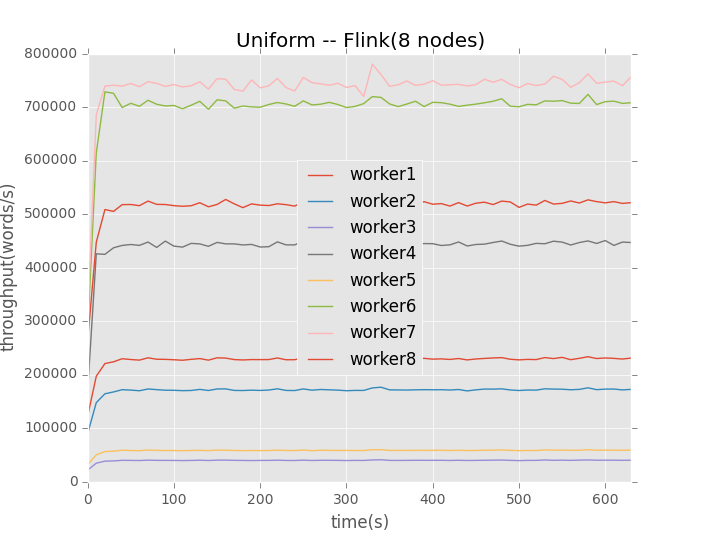
\includegraphics[scale=0.25]{images/flink_uniform_throughput}}

   \caption{Throughput of work nodes}
   \label{fig:worknodes_throughput}
  \end{center}
\end{figure}

\subsection{Online WordCount}
Base on the experiment results of Offline WordCount, we perform experiments of Online WordCount on Storm and Flink at half throughput of Offline WordCount respectively.  As mentioned in \cref{section:log_statistic}, the latency is computed as spending time from a record generated to corresponding result computed. Storm with ack enabled achieves a median latency of 10 milliseconds, and a 95-th percentile latency of 201 milliseconds, meaning that 95\% of all latencies were below 201 milliseconds. Flink has a litter higher median latency (53 milliseconds), and a 99-th percentile latency of 521 milliseconds that is close to Storm. 

\begin{figure}
  \begin{center}
  \subfigure{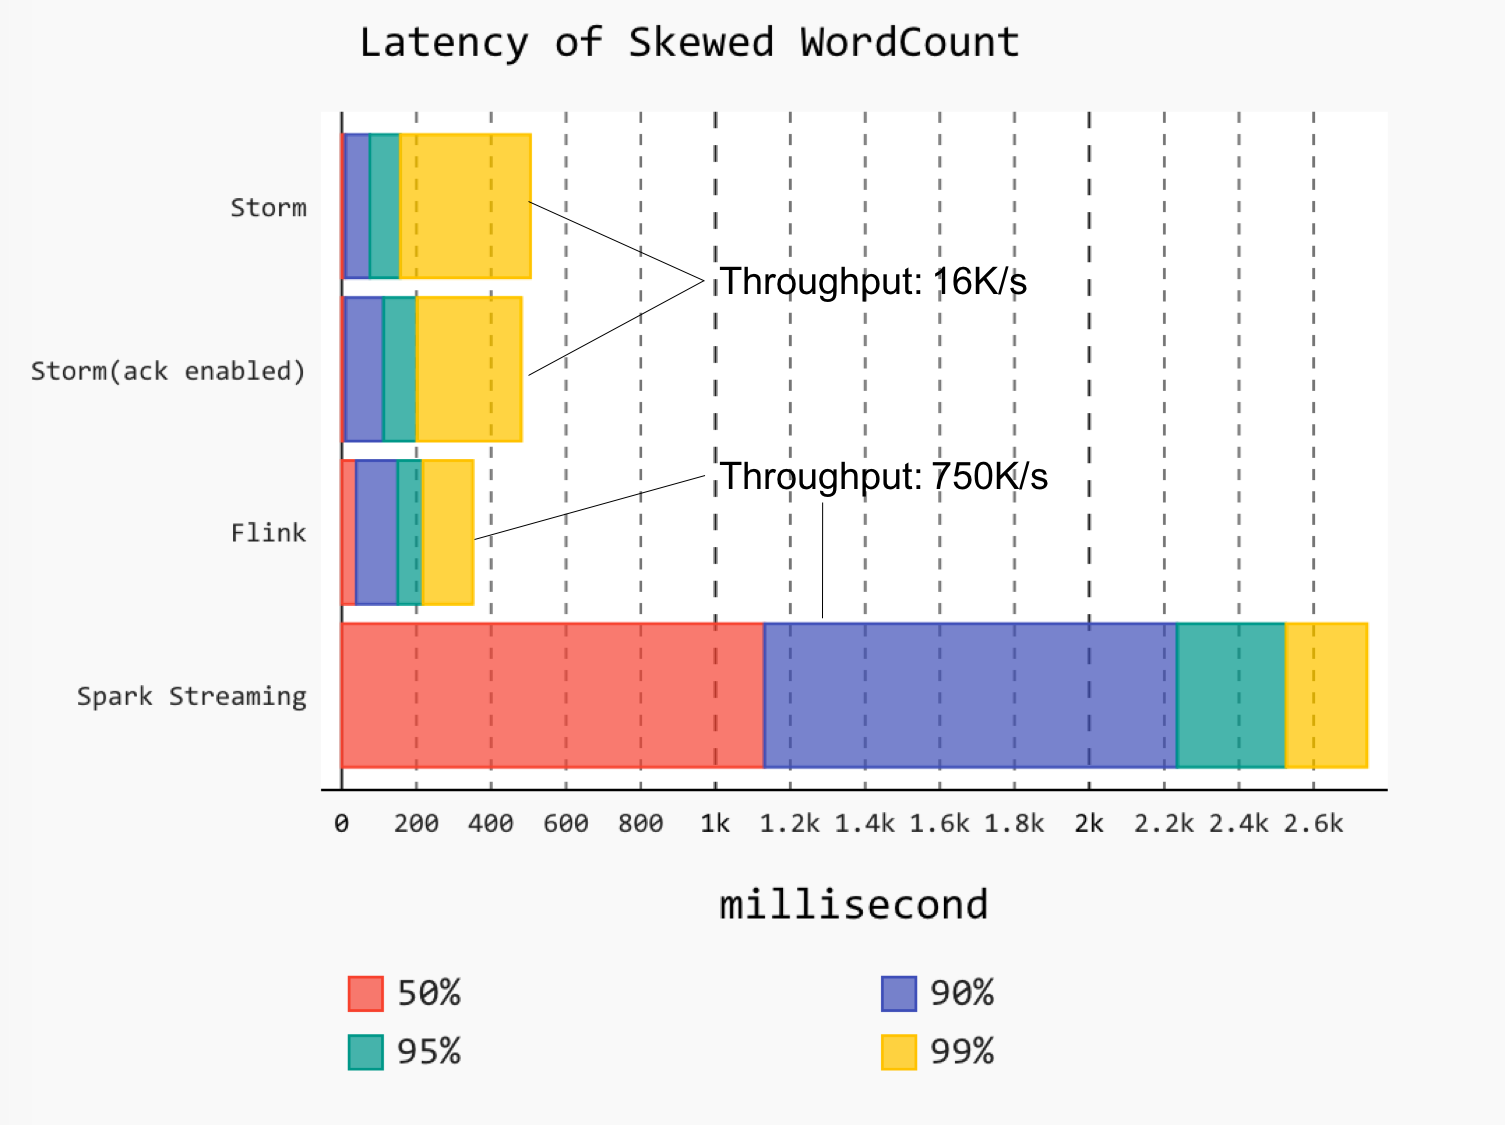
\includegraphics[scale=0.48]{images/latency_skewedwordcount}}
   \caption{Latency of Online WordCount}
   \label{fig:online_wordcount_latency}
  \end{center}
\end{figure}

In Spark Streaming, depending on the nature of the streaming computation, the batch interval used may have significant impact on the data rates that can be sustained by the application on a fixed set of cluster resources\footnote{\url{http://spark.apache.org/docs/1.5.1/streaming-programming-guide.html\#setting-the-right-batch-interval}}. Here, we perform the experiments with one second micro-batch interval and 10 seconds checkpoint interval which are the default configurations. Checkpointing is enabled because stateful transformation - updateStateByKey is used here to accumulate word counts.  Checkpointing is very time consuming because it needs to write information to a fault- tolerant storage system. Figure~\ref{fig:spark_wordcount_latency} shows that the latency of micro-batches processing increasing and decreasing periodically because of checkpointing. The throughput of experiment corresponding to Figure~\ref{fig:spark_wordcount_latency} is 1.4M/s (million words per second) of skewed data. When the speed of data generation reaches 1.8M/s, the delay and latency increase infinitely with periodic decreasing.

\begin{figure}
  \begin{center}
  \subfigure{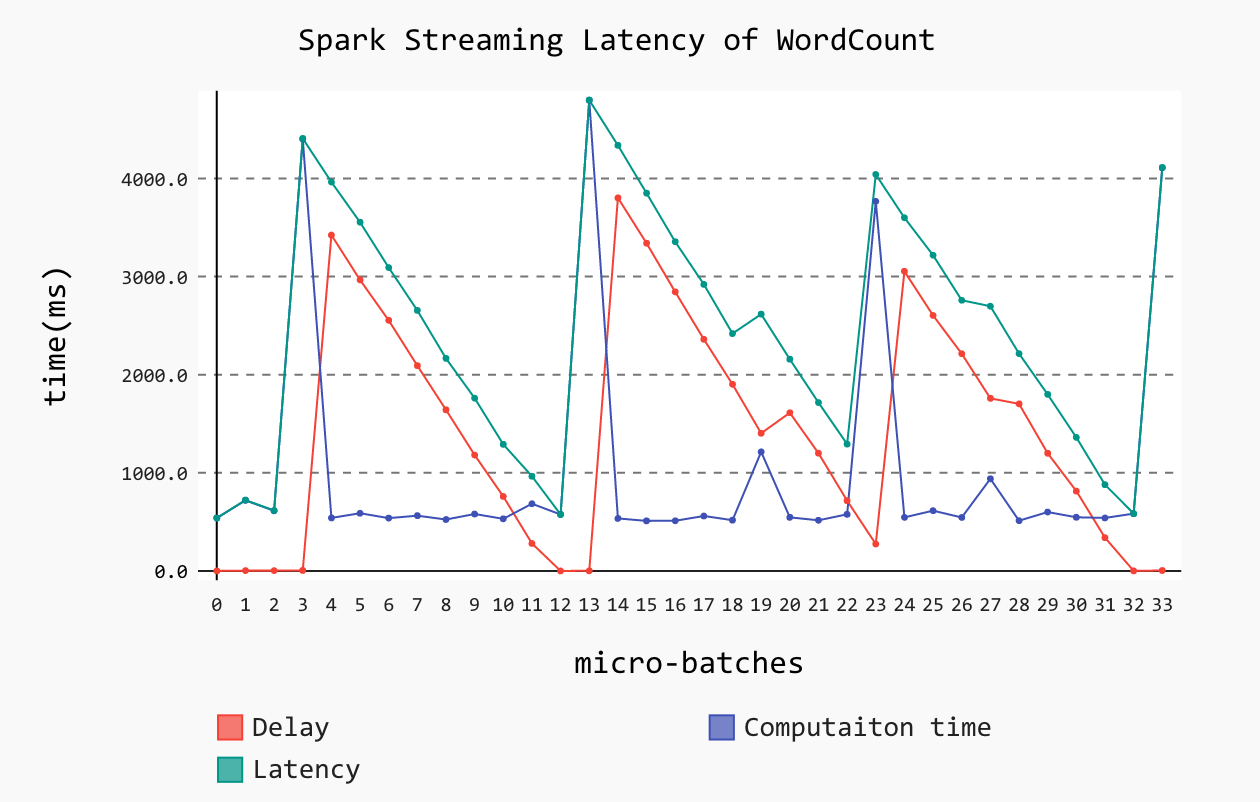
\includegraphics[scale=0.22]{images/spark_wordcount_latency}}
   \caption{Spark Streaming WordCount Latency}
   \label{fig:spark_wordcount_latency}
  \end{center}
\end{figure}


\subsection{Windowed WordCount}
\label{subsection:window_wordcount}

When dealing with skewed data, the compute node which count the word with largest frequency might be the bottleneck. Inspired from MapReduce Combiner, we designed another version of WordCount with \texttt{window} operator of stream processing. In reduce step, first words are shuffle grouped and applied pre-aggregation. Local pre-aggregation results are windowed for a configureable period. At last, the intermedia word counts are key grouped and reduced to get the final results. Actually, Spark Streaming supports pre-aggregation by default, and above Spark Streaming WordCount experiments already own this feature. Currently, Flink-0.10.1 doesn't support pre-aggregation and parallel window could only be applied on keyed stream. It is possible to implement Windowed WordCount with Flink's low level API. But it is too time consuming and we leave it to future works. Therefore, only Storm is benchmarked with this workload.

To support Windowed WordCount, we implemented a \texttt{window} operator in Storm\footnote{\url{https://github.com/wangyangjun/Storm-window}}. From our experiments, the window time has very limit effect on throughput. Here only experiment results of one second window workload are presented. The throughput of Offline WordCount performing skewed data could reach 60K/s (thousand words per second). While dealing with uniform data, the throughput doesn't have any obvious improvement. Online WordCount with 50K/s generation speed achieves a median latency of 1431 milliseconds, and a 99-th percentile latency of 3877 milliseconds.

\begin{figure}
  \begin{center}
  \subfigure{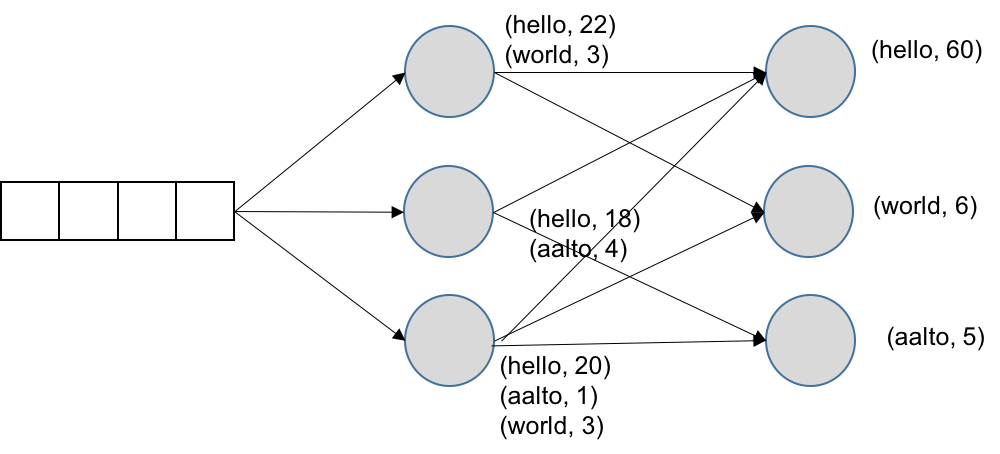
\includegraphics[scale=0.4]{images/window_wordcount}}
   \caption{Windowed WordCount}
   \label{fig:windowed_wordcount}
  \end{center}
\end{figure}



\section{Multi-Streams Join Workload}

\section{Iterate Workload}


\clearpage